
\section{Scope of Work and Objectives}
\label{scope}

\subsection{Scope of Work}
Biometric data indexing is a technique where an index key is generated for biometric
data and is assigned to the corresponding template. 
Based on these index keys the
biometric database can be categorized into groups of similar biometric templates.
This allows reducing the 1:N matching for identification purposes to a smaller set
of candidates for the query template. For a query image, the system will retrieve a
smaller set of candidate database templates to be matched with the query template,
which can effectively reduce the search and identification time. An overview of the indexing system is shown in Figure \ref{fig:steps_id}.
 
Biometric indexing can facilitate several biomteric-based systems such above mentioned FBI database of fingerprints, UIDAI's AADHAAR-based national identity system, as these systems are very large, and without a proper indexing mechanism in place, the identification process can be very inefficient. The Government of India has generated a
unique identity for each citizen through the biggest ever project called AADHAAR
under the aegis of Unique Identification Authority of India (UIDAI). The Central
Identity Data Repository (CIDR) in AADHAAR stores about 10+ Petabytes of data
 consisting of more than 1.33 billion people and their 13.3 billion fingerprints scans,
 2.66 billion iris scans, and 1.33 billion facial photos \cite{uidai}. For such a massive database, traditional indexing schemes fail, and thus there is a need for proper indexing mechanism for identification in large databases such as AADHAAR system.

 On surveying the existing literature, it is observed that there is a scope to further improve the performance of existing methods for key generation. 
 The robustness of the keys generated will affect the matching time taken when it uses that key as the index. 
 In order to achieve this, a sophisticated key generation method is needed.

 \begin{figure}[!ht]
    \centering
    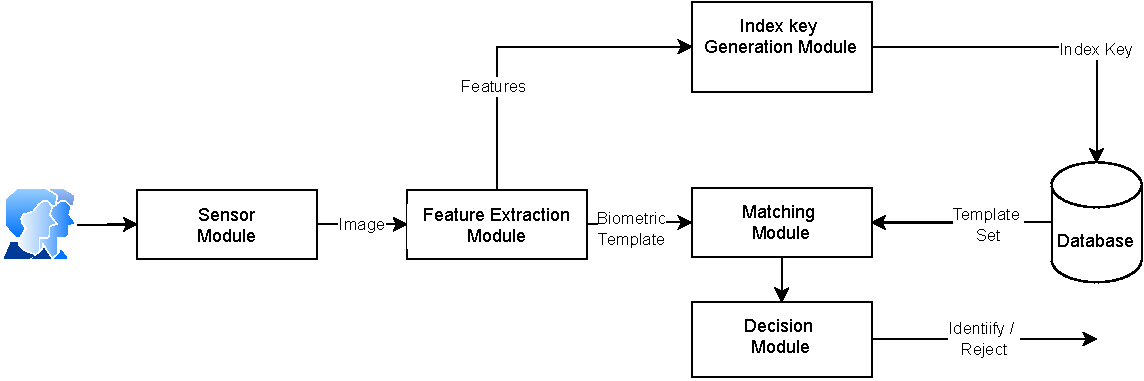
\includegraphics[width=0.85\textwidth]{images/steps_in_identification_with_indexing.drawio.pdf}
    \caption{Steps in Identification with Indexing}
    \label{fig:steps_id}
\end{figure}

\subsection{Motivation}
Identification suffers from two major limitations (a) false matching and (b) long response time due to a large candidate set. 
Traditional indexing schemes are not usable for indexing biometric databases as there is no numeric or alphabetical order in the biometric data.
In most of the previously proposed methods, there are certain shortcomings such as
\cite{Kavati2017} uses an extended triangulation-based method for indexing but the index vectors are
highly correlated which in turn causes the penetration rate to increase. In \cite{Bhanu2003} $O(N^3)$
triangles are used for generating index vectors which is computationally expensive.
In \cite{Germain1997}  they used texture-based global features for indexing, global texture features are not very robust against noise, core, and delta points may also not be present in
a fingerprint impression.
These shortcomings motivated this work to produce an effective indexing method
which is robust against noise, and also uses local features which are less expensive to
compute.

This work is mostly focused on creating an efficient indexing scheme for fingerprint
identification such that the penetration rate and false acceptance rate are reduced
and at the same time the identification accuracy is improved. This work uses image
enhancement to ensure stable minutiae point extraction.
 In this work, an effective way to compensate for the shortcomings of preexisting methods
for different modules is explored to find a better solution for the problem.

Considering only one trait for identification can prove fatal in many cases. Thus, there arises a necessity for multi-modal biometric systems which can resolve many identification issues. For such systems, similar multi-modal approach is needed in terms of indexing as well in order to ensure quick and efficient identification.

\subsection{Objectives}
The primary objective of this work is to propose an indexing scheme for different biometric traits which allows for fast retrieval and reduces the search space as well as search time. This work considers generating the index on individual traits as well as a combination of multiple biometric traits in order to improve performance, thereby ensuring that the penetration rate of the indexing scheme is fairly low with
reduced false matching to allow for secure and efficient identification. Along with the above, this work also aims to create an open-source dataset of various synthetic biometric trains for testing and comparing performances of different indexing mechanisms.
The objectives of the work are as follows:

\begin{enumerate}

    \item To create a large-scale virtual biometric dataset featuring low-quality and high-quality samples for multiple biometric traits (eg. Fingerprints, Iris, Face) as the first thesis objective. 
    The performance of traditional indexing schemes on the aforementioned synthetic data is to be evaluated and compared. 
    \item To design and implement an effective and scalable indexing scheme with distortion invariant features which enable large-scale biometric identification systems to reduce processing time in user identification in a uni-modal system as the second thesis objective.
    \item To design and implement an effective and scalable indexing scheme with distortion invariant features which enable large-scale biometric identification systems to reduce processing time in user identification in a multi-modal system as the final thesis objective.
    
% The index of the database will only be as strong as the key generated. This work proposes a novel approach to extracting features from a user's biometric data, as the second thesis objective.

% \item To ensure that the features used for indexing can not be reverse-engineered
% to generate the fingerprint data again. As the second objective of the thesis work, this work proposes a novel cryptographic key generation technique from the features extracted that is secure and non-invertible.

% \item  The key generated is used as an index to the biometric database. This work proposed an experimental procedure for testing and evaluating this index as the third objective of the thesis work.
\end{enumerate}